\subsection*{7.5\hspace*{0.5cm}Energy + Momentum - Question (Boulder)}
A 55.6 kg boulder sat on the side of a mountain beside a lake. The boulder was 14.6 m
above the surface of the lake. One winter
night, the boulder rolled down the mountain,
directly into a 204 kg ice-fishing shack that
was sitting on the frozen lake. What was the
velocity of the boulder and shack at the
instant that they began to slide across the
ice?
\subsection*{7.5\hspace*{0.5cm}Energy + Momentum - Graph and Givens}
\begin{minipage}{0.5\textwidth}
    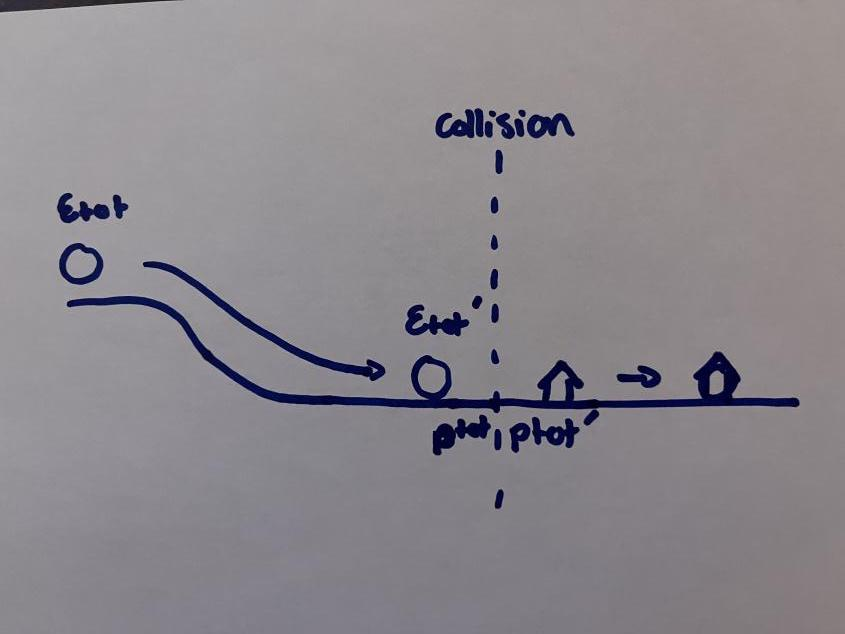
\includegraphics[scale=0.2]{./images/boulder.png}
\end{minipage}
\begin{minipage}{0.5\textwidth}
    \begin{itemize}
        \item $m_{b} = 55.6kg$
        \item $m_{s} = 204kg$
        \item $h_{b} = 14.6m$
        \item $h_{s} = 0m$
        \item $v_{bs} = ?$
    \end{itemize}
\end{minipage}
\subsection*{7.5\hspace*{0.5cm}Energy + Momentum - Solve}
Because the cart is not initially colliding with the spring, $E_{e}$ is zero. Because the cart's velocity post-collision is zero, $E_{k}$ is also zero. Because the cart and the spring are at the same height both before and after the collision, both $E_{g}$ and $E_{g}\prime$ are set to zero.\newline\newline
\textbf{1.} $E_{tot} = E_{tot}\prime$ \\
\begin{adjustwidth}{0.6cm}{0pt}
    $\cancelto{0}{E_{k}} + E_{g} = E_{k}\prime + \cancelto{0}{E_{g}\prime}$ \\\\
    $(m_{b})(g)(h_{b}) = \frac{1}{2}m_{b}v_{b}^2$ \\\\
    $\therefore v_{b} = \sqrt[]{\frac{(2)(m_{b})(g)(h_{b})}{m_{b}}} = \sqrt[]{\frac{(2)(55.6)(9.81)(14.6)}{(55.6)}} \approx 16.9\frac{m}{s}$
\end{adjustwidth}\vspace*{15pt}
\textbf{2.} $P_{tot} = P_{tot}\prime$ \\
\begin{adjustwidth}{0.6cm}{0pt}
    $m_{b}v_{b} + m_{s}\cancelto{0}{v_{s}} = m_{b + s}v_{bs}$ \\\\
    $\therefore v_{bs} = \frac{m_{b}v_{b}}{m_{b + s}} = \frac{(55.6)(16.9)}{(55.6 + 204)} \approx 3.61\frac{m}{s}$
\end{adjustwidth}\vspace*{15pt}